% include the figures path relative to the master file
\graphicspath{ {./content/analysis/figures} }

% \section{Segmentation method analysis}
\section{materials and methods (Segmentation method analysis)}

Thus, the set of queries that generate the pool of methodologies present in this work are available at the \emph{us-breast-lesion-delineation-survey}\todo{project website in github} open repository as scripts.
These queries screen all the publications included by targeted journals during the last 5 years for articles matching any of the search terms in order to build a bibliographic dataset. This dataset is complemented collecting all the articles that expand the citations tree, both forward and backwards, up to 2 levels. More details about this process can be found at the website of the project. Automatic criteria are used for rough pruning of the dataset while the final pruning has been carried out manually. Details of both are provided at the website.

\paragraph{Analysis of the methods}
\label{sec:intro:analysis_of_the_methods}
\added[id=sik]{
  Apart from the gathering of the papers to review, the analysis has been done in the following manner:
}
\begin{itemize}
  \item \added[id=sik]{the analysis is carried out in both bottom-up and top-down fashion}
  \item \added[id=sik]{using a generic corpora, key concepts from the selected articles are extracted using Rake algorithm.}
  \item \added[id=sik]{the key concepts are studied and they mainly cluster in four categories: (1) medical-breast related, (2) segmentation strategy, (3) evaluation, (4) other.}
  \item \added[id=sik]{highly cited articles in such topics are used to refine the initial corpora and update the key concepts of each paper for the bottom-up description.}
  \item \added[id=sik]{for the top-down strategy reference bibliography is used to drive the discussion of the articles key-concepts}
\end{itemize}


% \begin{table}[ht]
%   \caption{Query\todo{Query caption}}
%   \medskip
%     \begin{tabular}{r c}
%       % \toprule
%       token & keyword\\
%       % \midrule
%       organ: & breast \\
%       task: & segmentation, delineation, contouring \\
%       modality: & Ultrasound, Ultra-Sound, Ultrasonic, \\
%       & US image, Sonography, Sonograms \\
%       target publications: & %\todo{target publications}
%       % \bottomrule
%     \end{tabular}
%   \label{tab:query}
% \end{table}

\begin{table}[!ht]
\begin{adjustwidth}{-2.25in}{0in} % Comment out/remove adjustwidth environment if table fits in text column.
\caption{
{\bf Table caption Nulla mi mi, venenatis sed ipsum varius, volutpat euismod diam.}}
\begin{tabular}{|l|l|l|l|l|l|l|l|}
\hline
\multicolumn{4}{|l|}{\bf Heading1} & \multicolumn{4}{|l|}{\bf Heading2}\\ \hline
$cell1 row1$ & cell2 row 1 & cell3 row 1 & cell4 row 1 & cell5 row 1 & cell6 row 1 & cell7 row 1 & cell8 row 1\\ \hline
$cell1 row2$ & cell2 row 2 & cell3 row 2 & cell4 row 2 & cell5 row 2 & cell6 row 2 & cell7 row 2 & cell8 row 2\\ \hline
$cell1 row3$ & cell2 row 3 & cell3 row 3 & cell4 row 3 & cell5 row 3 & cell6 row 3 & cell7 row 3 & cell8 row 3\\ \hline
\end{tabular}
\begin{flushleft} Table notes Phasellus venenatis, tortor nec vestibulum mattis, massa tortor interdum felis, nec pellentesque metus tortor nec nisl. Ut ornare mauris tellus, vel dapibus arcu suscipit sed.
\end{flushleft}
\label{table1}
\end{adjustwidth}
\end{table}

\begin{figure}[!ht]
  \centering
  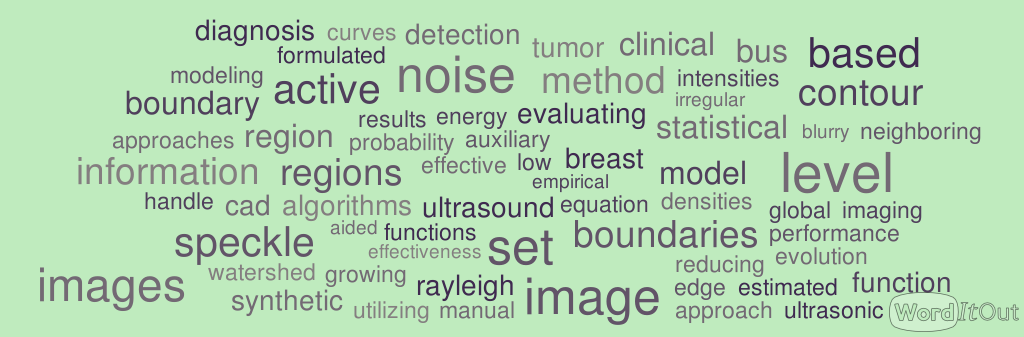
\includegraphics[width=0.8\textwidth]{./content/analysis/figures/wcloud.png}
    \caption{Word cloud representing the key-concepts generated from the bibliographic corpus.\todo{make a better wcloud clustering concepts and better key-concept detection}}
  \label{fig:wcloud}
\end{figure}

% Howto make a wordcloud 
% https://randomdeterminism.wordpress.com/2010/08/03/word-clouds-in-context/
